\documentclass[a4paper]{article}
\usepackage{polski}
\usepackage[utf8]{inputenc}

\usepackage{graphicx}    % Pakiet pozwalający ,,wklejać'' grafikę...

\usepackage{amsmath,amssymb,amsfonts,amsthm,mathtools}
                               % Dołączamy zestaw różnych przydatnych znaczków ...

% dane autora
\author{{\large Wiktor Pilarczyk}}
\title{\Huge Pracownia nr 0}
\date{\today}

% początek dokumentu
\begin{document}
\maketitle
\section{Podstway \LaTeX'a}

\subsection{Tabelka z liczbami}

\begin{center}
\begin{tabular}{|c|l|} \hline
Indeks & Liczba \\
\hline \hline
1 & 3.213\\
2 & 7.11111 \\
3 & 1.25 \\
4 & 5.1234 \\
5 & 4.3 \\
\hline
\end{tabular}
\end{center}

\subsection{Wykres}
\begin{figure}[h]
\centering
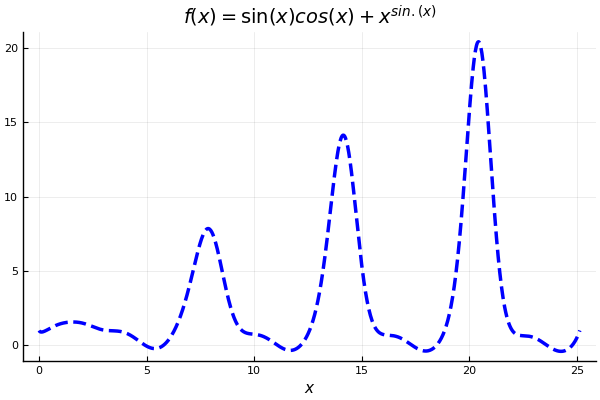
\includegraphics[width=12cm,height=7cm]{wykres.png}
\end{figure}
\section{Wzór Taylora}
\begin{equation}
f(x)= \sum_{k=1}^{n} \left(\frac{\left(x-a\right)^n}{k!}f^{(k)}(x) \right)+R_{n}(x,a)
\end{equation}
\thispagestyle{empty}
\end{document}
